%\documentclass{edm_template-no-copyright}
\documentclass{edm_template}
%\documentclass[11pt,twocolumn]{article}
\usepackage{amsmath}
\usepackage{graphicx}
\usepackage{flushend}
\usepackage{algorithmic}
%\usepackage{adjustbox}
\usepackage{paralist}
\usepackage{array}
\usepackage{apacite}
\usepackage{multirow}
\usepackage{dcolumn}
\usepackage{array}
\usepackage{kbordermatrix}
\usepackage{balance}
\usepackage{float}
\usepackage{xcolor}
\DeclareMathOperator*{\argmax}{arg\,max}
    
\newcommand{\Michel}[1]{{\textcolor{red}{[#1]}}}

\begin{document}

\title{An Empirical Research on Identifiability and Q-matrix Design for DINA model}
\numberofauthors{2}
\author{
\alignauthor
Peng Xu\\
       \affaddr{Polytechnique Montreal}\\
       \email{\large\sffamily peng.xu@polymtl.ca}
\alignauthor
Michel C. Desmarais\\
       \affaddr{Polytechnique Montreal}\\
       \email{\large\sffamily michel.desmarais@polymtl.ca}
}
\maketitle

\begin{abstract}
In most contexts of student skills assessment, whether the test material is administered by the teacher or within a learning environment, there is a strong incentive to minimize the number of questions or exercises administered in order to get an accurate assessment.  This minimization objective can be framed as a Q-matrix design problem: given a set of skills to assess and a fixed number of question items, determine the optimal set of items, out of a potentially large pool, that will yield the most accurate assessment.  In recent years, the Q-matrix identifiability under DINA/DINO models has been proposed as a guiding principle for that purpose.  We empirically investigate the extent to which identifiability can serve that purpose. Identifiability of Q-matrices is studied throughout a range of conditions in an effort to measure and understand its relation to student skills assessment.  The investigation relies on simulation studies of skills assessment with synthetic data.  Results show that identifiability is an important factor that determines the capacity of a Q-matrix to lead to accurate skills assessment with the least number of questions.
\end{abstract}

%%%%%%%%%%%%%%%%%%%%%%%%%%%%%%%%%%%%%%%%%%%%%%%%%%%%%%%%%%%%%%%%%%%%%%%%%%%%%
\section{Introduction}

% RQ: In this experiment, we only look at batch testing: assessment is based on the whole set of items.  But in adaptive testing, the choice of questions will depend on the current skills assessment.  Are the rules of identifiability for batch assessment the same as for adaptive testing?

Consider a set of items intended to assess a student's mastery over a set of skills, or knowledge components (KC).  These items, along with the set of skills, can be designed to test a single skill at once.  Or, they can be designed to involve two or more skills.  A test composed of a fixed number of items can either be composed of a mixture of single and multiple skills items, or composed of one type of items only.  Skills can themselves be defined so as to facilitate the creation of tasks/problems that involve single skill per item, or multiple skills per items.  By which principles should a teacher choose among these different options?

This paper addresses this question, with the general objective of designing a test that will bring the most accurate assessment of a student's skill mastery state with the least number of questions items.  

The investigation is framed within the DINA model, where question items can involve one or more skills, and where all skills are required to succeed the question, but a success can still occur through a guessing factor, and failure can also occur through a slip factor.  

%In adaptive testing, the goal is to ask the question items that are aligned with the student's estimated assessment and that will bring the most information, thereby increasing accuracy and reducing test length.  In a single skill framework, such as Item Response Theory (IRT), this goal is relatively well understood and straightforward. But in the case where multiple skills must be assessed simultaneously and where items can involve more than a single skill, the process is much more complex (see for eg.\ \citeNP{vie2017review}).  Assessment necessarily relies on how items relate to the skills we wish to assess.

%%%%%%%%%%%%%%%%%%%%%%%%%%%%%%%%%%%%%%%%%%%%%%%%%%%%%%%%%%%%%%%%%%%%%%%%%%%%%
\section{Q-matrix, DINA model and identifiability}

This mapping of items to skills is referred to as a Q-matrix, where items are mapped to latent skills whose mastery is deemed necessary in order for the student to succeed at the items.  An item can represent a question, an exercise, or any task that can have a positive or negative outcome.  In the DINA model, the conjunctive version of the Q-matrix is adopted.

In the last decade, considerable research has been devoted to deriving a Q-matrix from student test result data \cite{barnes2010novel, liu2012data, desmarais2015combining, xu2016boosted}.  Another line of research on Q-matrices has been devoted to refine or to validate an expert-given Q-matrix \cite{de2015general, chiu2013statistical, desmarais2013matrix}.

In parallel to these investigations around the derivation and refinement of Q-matrices, some researchers have looked at the question of the identifiability.  The general idea behind identifiability is that two or more configurations of model parameters can be considered as equivalent.  Sets of parameters will be considered equivalent if, for example, their likelihood are equal given a data sample.  Or, conversely, if the parameters are part of a generative model, two sets of equivalent parameters would generate data having the same characteristics of interest, in particular equal joint probability distributions (see~\citeNP{doroudi2017misidentified}, for more details).

The issue of identifiability for student skills assessment was first raised for the Bayesian Knowledge Tracing (BKT) model by \citeNP{beck2007identifiability} and later discussed by \citeNP{van2013properties}, and \citeNP{doroudi2017misidentified}.  In this paper, we consider the identifiability of the Q-matrix with regards to the DINA model, which was studied by \citeNP{xu2015identifiability} \citeNP{qin2015model}.  Detailed statistical analysis has been made under the DINA/DINO models, which was first discussed under the situation that slip and guess is zero \cite{chiu2009cluster}, and then the case that slip and guess exist but is known \cite{liu2013theory}, and finally the case that slip and guess is unknown \cite{chen2015statistical}. 

% However, how do we use the conditions offered by the discussion to guide our educational test? First, the discussion is centered around the identifiability on Q-matrix, not on the identifiability of students, which is also a critical problem \cite{beck2007identifiability}. Fortunately, for the case slip and guess are known, the identifiability of the parameters $p$ are also given \cite{chen2015statistical}.  

Identifiability is a general concept for statistical models. Its formal definition is:

\textbf{Definition} \cite{casella2002statistical} A parameter $\theta$ for a family of distribution ${f(x|\theta: \theta \in \Theta}$ is \textit{identifiable} if distinct values of $\theta$ correspond to distinct pdfs or pmfs. That is, if $\theta \neq \theta^{\prime}$, then $f(x|\theta)$ is not the same function of $x$ as $f(x|\theta^{\prime})$.

The DINA model has parameters $\theta = \{Q, p, s, g\}$, where $Q$ is the Q-matrix. $p$ is the categorical distribution parameter for the whole population. That is, it indicates the probability that a student belongs to each profile category. For example, in a 3-skill case, there are $2^3=8$ categories for students to belong to, and the 8-component probability vector of student belongs to each of these categories is the model parameter $p$. Finally, $s$ and $g$ are both vectors denoting the slip and guess of each item. 

The identifiability of all parameters in DINA model have been thouroughly investigated and several theorems are given \cite{xu2015identifiability}. But for the Q-matrix design problem that is the focus of this paper, we solely need to ensure that the model parameter $p$ is identifiable, meaning that we can distinguish different profile categories. Fortunately, for the case when $s$ and $g$ are known, the requirement easily satisfied, since it only requires the Q-matrix to be \textit{complete}.

\textbf{Definition} \cite{xu2015identifiability}  The matrix $Q$ is \textit{complete} meaning that $\{e_{i}:i=1,...k\} \subset R_{Q}$, where $R_{Q}$ is the set of row vectors of $Q$ and $e_{i}$ is a row vector such that the $i$-th element is one and the rest are zero.

And the heart of the current investigation is based on the following proposition:

\textbf{Proposition} \cite{xu2015identifiability} Under the DINA and DINO models, with $Q$, $s$ and $g$ being known, the population proportional parameter $p$ is \textit{identifiable} if and only if $Q$ is \textit{complete}.

%\Michel{What does this proposition imply exactly? That binary unit vectors are sufficient?}
   
%However, for Q-matrix related model, since exchanging columns does not yield an essentially different Q-matrix. During the research of \citeA{xu2015identifiability}, the identifiability of Q-matrix has been redefined.
%
%\textbf{Definition} \cite{xu2015identifiability} We write $Q \sim Q^{\prime}$ if and only if $Q$ and $Q^{\prime}$ have identical column vectors that can be arranged in different orders. We say that $Q$ is identifiable if there exists an estimator $\hat{Q}$ such that $\lim_{N\to\infty} P(\hat{Q} \sim Q) = 1$.

In the next section, we investigate empirically the Q-matrix design options in light of the \textit{completeness} requirement, using synthetic student performance data with the DINA model.  Synthetic data is essential for this investigation because we need to know the underlying ground truth and return to the issue of using real data in the conclusion.

%%%%%%%%%%%%%%%%%%%%%%%%%%%%%%%%%%%%%%%%%%%%%%%%%%%%%%%%%%%%%%%%%%%%%%%%%%%%%
\section{Experiment}
The Q-matrix design problem essentially is an optimization problem. Basically, we have a pool of Q-matrices, and each of them is formed by a selection with replacement from a pool of q-vectors. Each Q-matrix will yield some capacity to diagnose students, as measured by a loss function. We aim to choose a Q-matrix that minimizes the loss function.

In our experiments, to use Q-matrix to diagnose students under DINA model, we follow a Bayesian framework. First, we use one-hot encoding to denote all profile categories. Set $M$ to be the number of profile categories. Then, in 3-skill case, all the $M=8$ profile patterns $p_i$ in its original form is,

\kbordermatrix{
	& k_1 &k_2 & k_3\\
p_1 & 0 & 0 & 0 \\	
p_2 & 1 & 0 & 0 \\
p_3 & 0 & 1 & 0 \\
p_4 & 0 & 0 & 1 \\
p_5 & 1 & 1 & 0 \\
p_6 & 1 & 0 & 1 \\
p_7 & 0 & 1 & 1 \\
p_8 & 1 & 1 & 1 \\
}
and correspondent one-hot encodings are $\alpha_1=(1,0,0,0,0,0,0,0)$, $\alpha_2=(0,1,0,0,0,0,0,0)$,...,
$\alpha_8=(0,0,0,0,0,0,0,1)$.
%\Michel{This is confusing because $p_1$ appears as a row label, akin to the column label $k_1$, whereas it represents a probability distribution vector over the rows. Maybe use a notation such as $P(p_1)=(1,0,0,0,0,0,0,0)$, $P(p_2)=(0,1,0,0,0,0,0,0)$,...,$P(p_8)=(0,0,0,0,0,0,0,1)$ ?}
Then, we set the prior of each student profile to be 

$\alpha_0=(1/8,1/8,1/8,1/8,1/8,1/8,1/8,1/8)$ 

With the conditional independence assumed(i.e, conditioned on a given profile category, the probability to answer each question correct is independent), the likelihood is given by \cite{de2009dina}
$$ L(\alpha|X) = P(X|\alpha) = \prod_{i=1}^I P(X_i|\alpha_i) = \prod_{j=1}^J P_j(\alpha_i)^{X_{ij}}[1-P_j(\alpha_i)]^{1-X_{ij}}$$
in which $X$ is the response matrix and $X_i$ is the $i$-th row, $I$ is the number of records(students), $J$ is the  number of questions. $P_j(\alpha_i)$ is the probability of student profile $\alpha_i$ to answer correctly of question $j$, which is given by DINA model
$$ P_j(\alpha_i) = P(X_{ij}=1|\alpha_i)=g_j^{1-\eta_{ij}}(1-s_j)^{\eta_{ij}}$$
and posterior $\hat{\alpha}$ for each student will be calculated based on likelihood and prior. It will have the form
$$\hat{\alpha} = (m_1,m_2,m_3,m_4,m_5,m_6,m_7,m_8)$$ 
and then we calculate the loss between this posterior and the true profile $\alpha_{\mathrm{true}}$, which is one of the one-hot encoding vector. 

In short, for any Q-matrix configuration, the loss function is defined as
\newcommand\norm[1]{\left\lVert#1\right\rVert}
$ loss(Q) = \sum_{\mathrm{students}} \norm{\hat{\alpha} - \alpha_{\mathrm{true}}}^2$ 

To implement the experiment, for each Q-matrix configuration, we will generate a response matrix based on DINA model given fixed slip and guess parameters, using function 'DINAsim' from R package 'DINA' \cite{Culpepper2015}, then calculate the posterior estimation for all students and evaluate the total loss. The reported result is an average loss of 100 runs. 

In our experiments, we consider the 3-skills case and 4-skills case respectively. For 3-skills case, we conduct it with $N=200$ students, of which 25 students falling into each of 8 categories. For 4-skills case, we conduct it with $N=400$ students, of which 25 students falling into each of 16 categories. 

\subsection{Experiment 1: Comparison of three strategies}
In the first experiment, we compare three different Q-matrix design strategies. They are all based on repetition of a specific pool of q-vectors.
\begin{itemize}
\item Strategy 1: Using the identifiability condition by only repeatedly using the vectors $\{e_{i}:i=1,...k\}$. Q-matrix used in this strategy is denoted as Q-matrix~1.
\item Strategy 2: Using the vectors $\{e_{i}:i=1,...k\}$ plus a all-one vector $(1,1,1)$ or $(1,1,1,1)$. This is inspired by orthogonal array design, which is a commonly seen design of experiments \cite{montgomery2017design}. Q-matrix used in this strategy is denoted as Q-matrix~2.
\item Strategy 3: Repeatedly using all q-vectors. Q-matrix used in this strategy is denoted as Q-matrix~3.
\end{itemize}
For the 3-skills case, all these three Q-matrices are shown below. The general pattern is to recycle the rows above the lines denoted~$q_i [..., ..., ...]$.

\parbox{.5\columnwidth}{
\centering
Q-matrix 1\\
\vspace*{-1ex}
\kbordermatrix{
	& k_1 &k_2 & k_3\\
q_1 & 1 & 0 & 0 \\
q_2 & 0 & 1 & 0 \\
q_3 & 0 & 0 & 1 \\
... & ... & ... & ... &\\
q_{19} & 1 & 0 & 0 \\
q_{20} & 0 & 1 & 0 \\
q_{21} & 0 & 0 & 1 \\
}
\vspace*{2ex}
{Q-matrix 2}\\
\vspace*{-1ex}
\kbordermatrix{
	& k_1 &k_2 & k_3\\
q_1 & 1 & 0 & 0 \\
q_2 & 0 & 1 & 0 \\
q_3 & 0 & 0 & 1 \\
q_4 & 1 & 1 & 1 \\
... & ... & ... & ... &\\
q_{17} & 1 & 0 & 0 \\
q_{18} & 0 & 1 & 0 \\
q_{19} & 0 & 0 & 1 \\
q_{20} & 1 & 1 & 1 \\
q_{21} & 1 & 0 & 0 \\
}}
\parbox{.5\columnwidth}{
\centering
{Q-matrix 3}\\{(all~combinations)} \\
\kbordermatrix{
	& k_1 &k_2 & k_3\\
q_1 & 1 & 0 & 0 \\
q_2 & 0 & 1 & 0 \\
q_3 & 0 & 0 & 1 \\
q_4 & 1 & 1 & 0 \\
q_5 & 1 & 0 & 1 \\
q_6 & 0 & 1 & 1 \\
q_7 & 1 & 1 & 1 \\
... & ... & ... & ... &\\
q_{15} & 1 & 0 & 0 \\
q_{16} & 0 & 1 & 0 \\
q_{17} & 0 & 0 & 1 \\
q_{18} & 1 & 1 & 0 \\
q_{19} & 1 & 0 & 1 \\
q_{20} & 0 & 1 & 1 \\
q_{21} & 1 & 1 & 1 \\
}}

The 4-skills case is similar, which is omitted here. Results of these two cases are shown in Figure ~\ref{fig:ComparisonThreeSkill} and Figure~\ref{fig:ComparisonFourSkill}.

\subsection{Experiment 2: Find best configuration}
The second experiment takes the brutal force approach. We directly examine all possible Q-matrix configurations. First, for a given pool of q-vectors to choose from and an integer indicating the number of questions, we need to know the number of possible configurations of Q-matrices we have. This is equivalent to a classical combinatorial problem, that is, to allocate distinguished balls(q-vectors) to indistinguished cells(questions). It can be easily computed by combinatorial coefficients and interpreted by using stars and bars methods. For example, in 3-skills case, we have 7 q-vectors, and if we have 4 questions to allocate them, then we have ${{4+7-1}\choose {7-1}}=210$ possible configurations. This number grows up sharply as number of questions increases or number of patterns increases. As a comparison, in the 4-skills case, if we have 5 questions to allocate them, then we have ${{5+15-1}\choose {15-1}}=11628$ possible configurations. 

For each configuration, we will calculate the MAP estimation for all categories of each student, and compare with the one-hot encoding for their true categories. The total loss is reported as the performance index.

We show the results of 6 combinations of different numbers of skills and questions: 
\begin{itemize}
\item 3-skills case, 4 questions: Figure~\ref{fig:theta001J4ThreeSkill}, Figure~\ref{fig:theta021J4ThreeSkill}
\item 3-skills case, 8 questions: Figure~\ref{fig:theta001J8ThreeSkill}, Figure~\ref{fig:theta03J8ThreeSkill}
\item 4-skills case, 5 questions: Figure~\ref{fig:theta001J5FourSkill}, Figure~\ref{fig:theta02J5FourSkill}
\end{itemize}

%\Michel{Explain the strategies here and say a word about the DINA slip and guess (maybe report the formula of the DINA model in the section where it is presented?)}

\section{Result}
All results are given in form of figures.
\begin{figure}[h!]
  \begin{center}
  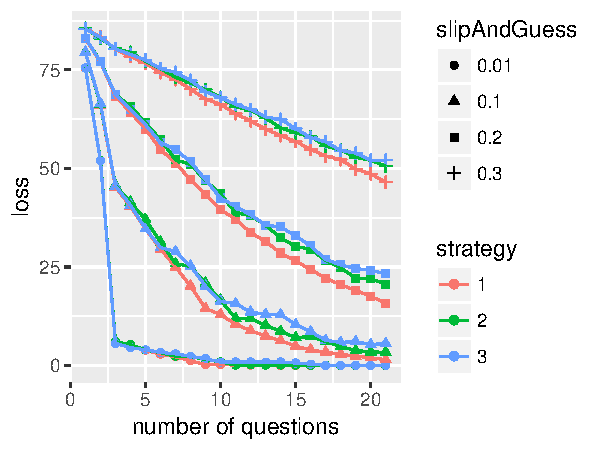
\includegraphics[width=\columnwidth]{simResults/LossStrategyComparisonThreeSkills.pdf}
  \end{center}
  \caption{Three Strategy Comparison on 3-skills case}  
  \label{fig:ComparisonThreeSkill}
\end{figure}

\begin{figure}[h!]
  \begin{center}
  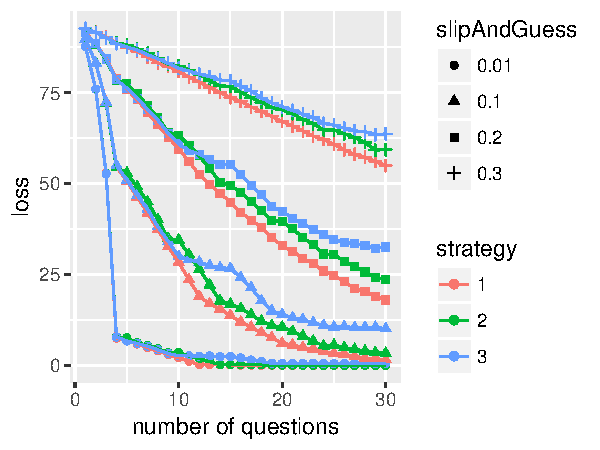
\includegraphics[width=\columnwidth]{simResults/LossStrategyComparisonFourSkills.pdf}
  \end{center}
  \caption{Three Strategy Comparison on 4-skills case}  
  \label{fig:ComparisonFourSkill}
\end{figure}

\begin{figure}[h!]
  \begin{center}
  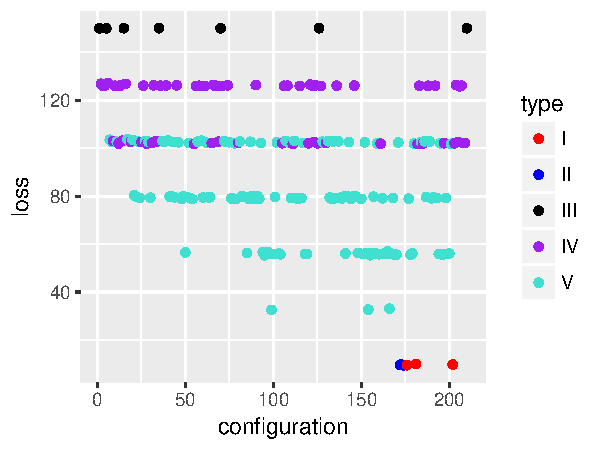
\includegraphics[width=\columnwidth]{simResults/LossBestConfig_theta001_J4.pdf}
  \end{center}
  \caption{3-skills case, slip=guess=0.01, J=4}  
  \label{fig:theta001J4ThreeSkill}
\end{figure}

\begin{figure}[h!]
  \begin{center}
  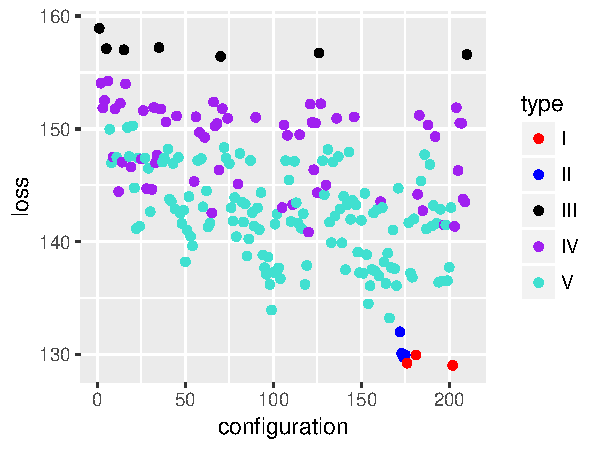
\includegraphics[width=\columnwidth]{simResults/LossBestConfig_theta02_J4.pdf}
  \end{center}
  \caption{3-skills case, slip=guess=0.2, J=4}  
  \label{fig:theta021J4ThreeSkill}
\end{figure}

\begin{figure}[h!]
  \begin{center}
  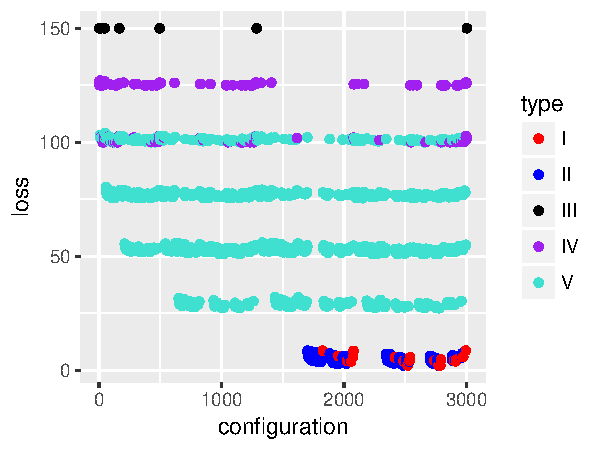
\includegraphics[width=\columnwidth]{simResults/LossBestConfig_theta001_J8.pdf}
  \end{center}
  \caption{3-skills case, slip=guess=0.01, J=8}  
  \label{fig:theta001J8ThreeSkill}
\end{figure}

\begin{figure}[h!]
  \begin{center}
  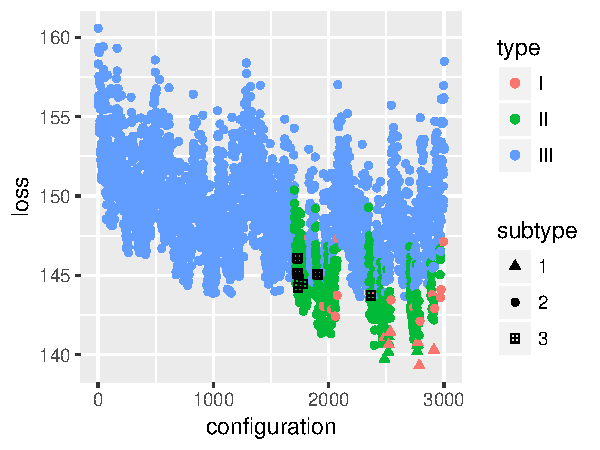
\includegraphics[width=\columnwidth]{simResults/LossBestConfig_theta03_J8.pdf}
  \end{center}
  \caption{3-skills case, slip=guess=0.3, J=8}  
  \label{fig:theta03J8ThreeSkill}
\end{figure}

\begin{figure}[h!]
  \begin{center}
  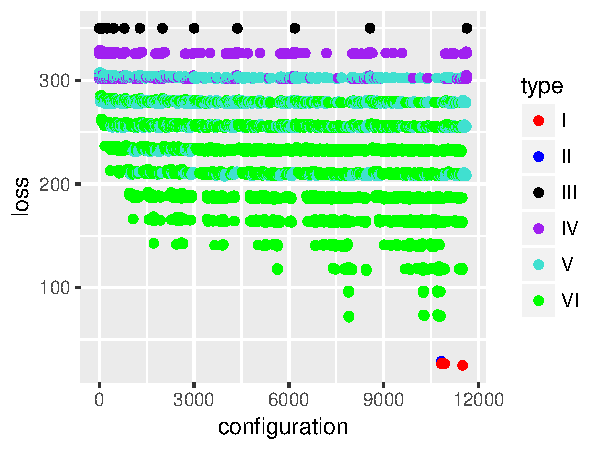
\includegraphics[width=\columnwidth]{simResults/Skill4LossBestConfig_theta001_J5.pdf}
  \end{center}
  \caption{4-skills case, slip=guess=0.01, J=5}  
  \label{fig:theta001J5FourSkill}
\end{figure}

\begin{figure}[h!]
  \begin{center}
  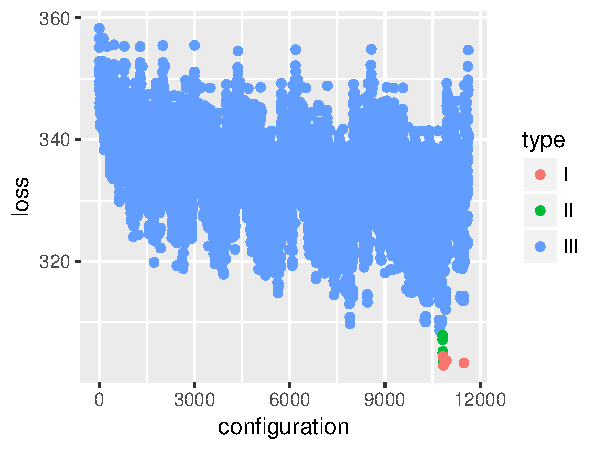
\includegraphics[width=\columnwidth]{simResults/Skill4LossBestConfig_theta02_J5.pdf}
  \end{center}
  \caption{4-skills case, slip=guess=0.2, J=5}  
  \label{fig:theta02J5FourSkill}
\end{figure}

%\begin{figure}[htbp]
%  \centering
%  \includesvg{theta02J5Total}
%  \caption{svg image}
%\end{figure}

\section{Discussion}
From the result in experiment 1 we can see that strategy 1 always works better than the other two strategies, meaning that by simply repeating the vectors $\{e_{i}:i=1,...k\}$ in Q-matrix design, without using any combination of skills yields better performance in student diagnosis. %\Michel{you mean binary unit vectors? I guess once you explain the strategies it should be clear.}

From the result in experiment 2, when slip and guess parameters are as low as 0.01, we can see obvious graded patterns among different configurations. This can be explained by the distinguishability of Q-matrix. For example, in Figure~\ref{fig:theta001J4ThreeSkill}, we can see there are 7 layers. In fact, the first layer consisted of Q-matrix that can only cluster students into 2 categories. One example of such kind Q-matrix is
\kbordermatrix{
	& k_1 &k_2 & k_3\\
q_1 & 1 & 0 & 0 \\	
q_1 & 1 & 0 & 0 \\
q_1 & 1 & 0 & 0 \\
q_1 & 1 & 0 & 0 \\
}

This Q-matrix can only discriminate between a student that mastered skill 1 or not. We know that there are in fact 8 categories of students, the 7 layers in Figure~\ref{fig:theta001J4ThreeSkill} from top to bottom correspond to the Q-matrix that can separate students into 2 to 8 categories. We can see that complete Q-matrix always fall in the bottom layer, which concurs with the proposition of Section~2. The 4-skills case is similar in Figure~\ref{fig:theta001J5FourSkill}.

When slip and guess parameter increase, it makes the points becomes more divergent which can be easily seen by comparison between Figure~\ref{fig:theta001J4ThreeSkill} and Figure~\ref{fig:theta021J4ThreeSkill}. In order to see some more details, we distinguish three types of Q-matrices. 
\begin{itemize}
\item Type I: Complete and confined, meaning it is only consisted of vectors $\{e_{i}:i=1,...k\}$.
\item Type II: Complete but not confined, meaning it not only contains all vectors $\{e_{i}:i=1,...k\}$, but also contains at least one other q-vector.
\item Type III: Incomplete Q-matrix.
\end{itemize}
Type I and Type II Q-matrices performs the same when slip and guess are low (Figure~\ref{fig:theta001J4ThreeSkill}, Figure~\ref{fig:theta001J5FourSkill}), but when they get higher, Type II Q-matrices show a better performance (Figure~\ref{fig:theta021J4ThreeSkill}, Figure~\ref{fig:theta02J5FourSkill}).

However, when more questions are involved in high slip and guess, the performance becomes more unstable. Therefore, we again consider more subtypes. In 3-skills case for 8 questions, we consider three subtypes below. 
\begin{itemize}
\item Subtype 1: Q-matrix contains each component of $\{e_{i}:i=1,...k\}$ at least twice. 
\item Subtype 2: Other situation (e.g A complete Q-matrix but all the other vectors are just repeated $e_1$).
\item Subtype 3: Q-matrix contains all q-vectors.
\end{itemize}
From Figure~\ref{fig:theta03J8ThreeSkill} we can see that the subtype 1 (denoted by triangle) shows better performance than subtype 2, meaning that repeating the whole complete Q-matrix is a better strategy just like the strategy 1 we used in experiment 1. Subtype 3 corresponds to the strategy 3 in experiment 1, it has only 7 possible configurations in 8-question setting and we can see that they do not perform well.

Therefore, we argue that the best Q-matrix design is to use only the vectors $\{e_{i}:i=1,...k\}$ since it offers quicker convergence speed (as shown in experiment 1) and better robustness against slip and guess (as shown both in experiment 1 and 2).

%%%%%%%%%%%%%%%%%%%%%%%%%%%%%%%%%%%%%%%%%%%%%%%%%%%%%%%%%%%%%%%%%%%%%%%%%%%%%
\section{Conclusion}

This work is still in an early stage and has limitations, in particular because it is conducted with synthetic data, but the main finding is wide reaching and warrants further investigations.  The support for desining Q-matrices that satisfy the identifiability condition by single-skill items is compelling in the experiments conducted with synthetic data.  The results clearly show such matrices yield more accurate student skills assessment. In particular, they show that Q-matrices that contains items that span the whole range of potential combinations of skills tend to yield lower skills assessment than Q-matrices that simply repeat the pattern of single-skill items.

The finding that tests composed of single-skill items are better for skills assessment is somewhat counter-intuitive, as intuition suggests that a good test should also include items with combinations of skills.  But intuition also suggests that items that involve combination of skills are more difficult, and it may not simply be because they involve more than one skill.  It might be that solving items that combine different skills in a single problem is a new skill in itself.  This conjecture is in fact probably familiar to a majority of educators, and the current work provides formal evidence to support it.  And the immediate consequence is that Q-matrices, as we currently conceive them, fail to reflect that a task that combines skill involves a new skill.

Ideally, future work should be conducted with real data.  However, given that we do not know the real Q-matrix that underlies real data, investigating the questions raised by the current study is non trivial.  Meanwhile, further experiments with synthetic data can be considered with different choice on student profiles distribution, and different number of skills involved. Besides, the case where slip and guess are unknown should also be considered, which involves a different identifiability requirement \cite{xu2015identifiability}. 

\bibliographystyle{apacite}
\bibliography{biblio}

\end{document}